%!TEX root = physical_authent.tex
As mentioned in the introduction, the protocol must ensure that only a genuine verifier can exploit the leakage from a prover, while avoiding any attacker attempting to mount a side-channel analysis. It must also consider some practical constraints such as the use of standard cryptographic APIs (\emph{i.e.} avoiding customized AES implementations as required in \cite{SakiyamaMMKHMMN15} for instance). 

\subsection{Adversarial Model}
In the sequel, we shall consider the following assumptions.
\begin{assumption}[\textbf{Attacker's profile}]
\label{assump_1}
We consider an attacker who can perform $(1)$ side-channel attacks by capturing the side-channel leakage of the prover to try retrieving the secret key and $(2)$ relay attacks to try authenticating to a verifier as a genuine prover. 
\end{assumption}


\begin{assumption}[\textbf{Impracticability of reproducing the physical leakage}]
\label{assump_2}
We assume that it is significantly difficult in practice for an attacker performing a relay attack to generate a copy of the side-channel information leaked by the genuine prover. This assumption is quite realistic and is merely justified in Sec.~\ref{ssec:security}.
\end{assumption}


Assumption~\ref{assump_2} relies on the fact that even if an attacker succeeds in capturing, copying and replaying the side-channel leakage, then this procedure will take some time denoted $\Delta$. Thus, replaying the side-channel information is equivalent to add some desynchronization in the trace which is well known to reduce the degree of correlation~\cite{DBLP:books/daglib/0017272}.


\subsection{Protocol Specification}
\label{sec_proposal}
\subsubsection{Overall Description.}\label{sssec:overall}
We provide in Fig.~\ref{fig:protocol} an overview of our protocol. 
First, we assume that the master key $K$ has already been shared between the verifier and the prover (\emph{e.g.} either loaded during the personalization phase of the prover or by using the classical Diffie-Hellman key exchange protocol with certified public keys on both sides).
\add{The prover initiates the protocol by sending $R_P$ (a $128$-bit random value) to the verifier who replies by sending $R_V$ (a $128$-bit random value). Both then use $R_V\oplus R_P$ (as an alternative one could use $R_V||R_P$)} as an input to a secure \textit{Key Derivation Function}, denoted KDF in Fig.~\ref{fig:protocol}, to generate $2N$ session keys $(K_0^{(0)}, K_1^{(0)}, \cdots, K_{2N-1}^{(0)}) = (K_0, K_1, \cdots, K_{2N-1})$ using the shared master key $K$.
This secure KDF (\emph{i.e.} orange box in Fig.~\ref{fig:protocol}) must be protected against classical side-channel attacks by implementing for instance some well-known masking countermeasures (see \emph{e.g.}~\cite{DBLP:conf/eurocrypt/Coron14,DBLP:conf/ches/GenellePQ11,DBLP:conf/ches/RivainP10}). In addition, the verifier generates $q \times 2N$ extra random keys denoted $(K_0^{(i)}, K_1^{(i)}, \dots, K_{2N-1}^{(i)})$ for $i \in [1,q]$. Now, to fix the practical issues of the protocol proposed in \cite{SakiyamaMMKHMMN15}, we use a set of $N$ AES encryption (\emph{i.e.} the 	blue boxes in Fig.~\ref{fig:protocol}) instead of a customized $N$-round AES. 
These AES executions, denoted \textit{leaky AES} in the sequel, do not implement any countermeasure against side-channel analysis and are used to encipher the last $N$ session keys

$(K_N, \cdots, K_{2N-1})$ using the first $N$ ones $(K_0, K_1, \cdots, K_{N-1})$ as encryption keys.\newline
On the prover side, the $i^{\text{th}}$ AES encryption provides $C_i = \mbox{AES}_{K_i}(K_{i+N})$ and leaks all intermediate sensitive variables which are measured by the verifier.

The verifier on its side, computes $q+1$ such sequences of $N$ AES and stores all relevant intermediate sensitive variables. The $j^\text{th}$ output of the $i^\text{th}$ sequence of $N$ AES is denoted $C_j^{(i)} = \mbox{AES}_{K_j^{(i)}}(K_{j+N}^{(i)})$ for $j$ in $[0,N-1]$ and $i$ in $[0,q]$.
Then, for each $i^\text{th}$ executed sequence of $N$ AES, the verifier computes a likelihood value $\mathcal{L}_i$ between the corresponding stored intermediate values and the acquired measurement while the prover was executing its $N$ leaky AES.

At the end of this step, the verifier holds $q+1$ likelihood values $\mathcal{L}_i$ with $i$ in $[0, q]$.
If the prover is genuine, then the maximum value of likelihood should be $\mathcal{L}_0$ (since obtained using the  session keys derived from the shared master key $K$) and a gap should exist between $\mathcal{L}_0$ and $\{\mathcal{L}_{i}\}_{i\in [1,q]}$ (denoted $\{\mathcal{L}_{i\not=0}\}$ in the sequel).
If the greatest likelihood value is not $\mathcal{L}_0$ or if $\mathcal{L}_0$ does not stand out from $\{\mathcal{L}_{i\not=0}\}$, then the authentication is rejected and the protocol ends.
Otherwise, the verifier continues the protocol by sending the ciphertext $C_k^{(0)}$ where $k$ is chosen randomly in $[0, N-1]$.

Upon receiving $C_k^{(0)}$, the prover checks whether it belongs to the set of ciphertexts it has computed (\emph{i.e.} whether it exists $l$ in $[0, N-1]$ \emph{s.t.} $C_l = C_k^{(0)}$) and if so, sends back a different ciphertext $C_m$ (\emph{i.e.} $ m \neq l$). Otherwise, the prover rejects the authentication. The verifier finally checks whether it holds $C_l^{(0)}$ such that $C_l^{(0)} = C_m$. If it is the case the verifier and the prover are mutually and physically authenticated.

\begin{figure}[ht!]
   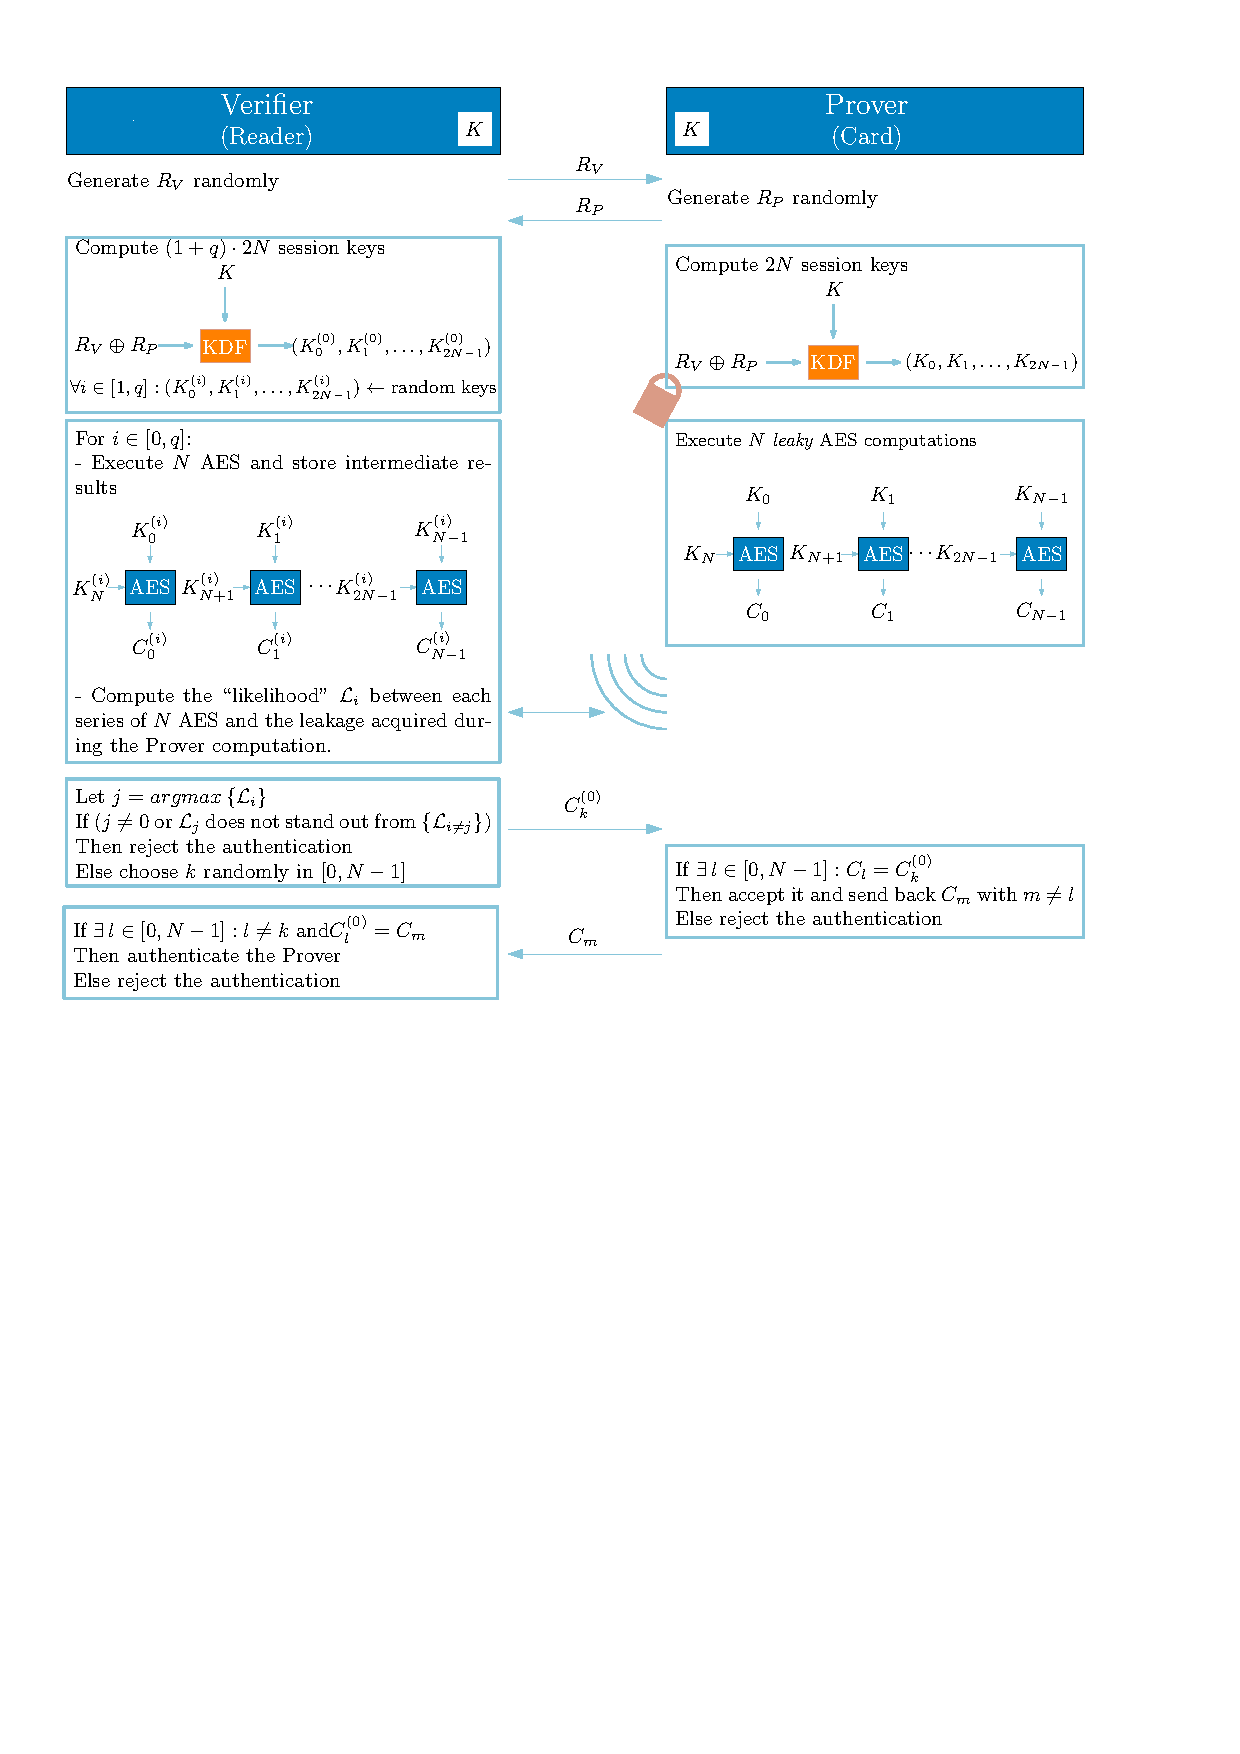
\includegraphics[width=1.0\linewidth]{../pics/protocol_2N-1.pdf}
   \caption{Description of the physical authentication protocol.} \label{fig:protocol}
\end{figure}

The most critical step for the success of our protocol is the acquisition of the physical leakage since it requires a perfect synchronization between the prover and the verifier.
To ensure this, a trick would consist in triggering a timer, at the verifier side, upon sending the random value $R_V$. This timer considers the round-trip time between the prover and the verifier and the averaged time of executing the secure AES at the prover side. When the timer expires, the acquisition starts.  
Then, from the collected measurement the verifier needs to select the so-called Points Of Interest (POI) by applying some well-known selection algorithms (\emph{e.g.}~\cite{Choudary2014,Friedman:1974,DBLP:conf/ches/StandaertA08}).
Following notations from Sec.~\ref{ssec:AES}, the verifier can target all the following bytes of AES states\footnote{ShiftRows is not considered since it is simply a rearrangement of the AES state thus providing no additional information.}:

\begin{equation}\label{eq:bytes}
\left.
\begin{array}{lcl}
\mbox{AddRoundKey: }& &  X_r[l,c]\\
\mbox{SubBytes: }  & & {Y_r[l,c]}\\
\mbox{MixColumns:  }& & {M_r[l,c]}
\end{array}\right\} \mbox{for } 0 \leq r \leq N_r - 1 \mbox{ and } (l,c) \in \{0,\cdots,3\}^2
\end{equation}



Thus, each AES execution gives rise to $(3 \times 16 \times N_r)$ different sensitive byte variables along its execution. Each byte variable leaks following the same generic model (see Equation~\eqref{eq:leak}) but instantiated with different model parameters (\emph{i.e.} different pairs of $(\alpha_t, \beta_t)$). Fortunately, it has been proven and confirmed experimentally that each sensitive byte variable leaks following the same model with the {\it same} parameters across the $N$ AES executions. 

\subsubsection{Likelihood Computation.}

Following the notations from Algorithm~\ref{alg:AES}, let $\{ {(X_r^{(j)}, Y_r^{(j)}, M_r^{(j)})}_{0 \leq r \leq N_r - 1}\}$ be the set of internal states that the verifier predicts, round by round, when executing the $j^{\text{th}}$ AES of the $i^{\text{th}}$ set of N AES execution, \emph{i.e.} $C_j^{(i)} = \mbox{AES}_{K_j^{(i)}}(K_{N+j}^{(i)})$.
After computing the whole $i^{\text{th}}$ set of $N$ AES, the verifier holds $\{{(X_r^{(j)}, Y_r^{(j)}, M_r^{(j)})}_{(0 \leq r \leq N_r - 1) \times (0\leq j \leq N-1)}\}$. 
The computation of the $i^{\text{th}}$ likelihood $\mathcal{L}_i$ can be executed following the paradigm illustrated in Algorithm~\ref{alg:likelihood}. 

\begin{algorithm}[ht!]
	\caption{Computation of the $i^{\text{th}}$ likelihood $\mathcal{L}_i$}\label{alg:likelihood}
	\begin{algorithmic}[1]
	\Require{$\{{(X_r^{(j)}, Y_r^{(j)}, M_r^{(j)})}_{(0 \leq r \leq N_r - 1) \times (0\leq j \leq N-1)}\}$: the intermediate values, $T$: the acquired trace}
  %$(T_0, T_1, \cdots, T_{N-1})$: the acquired traces}
	\Ensure{$\mathcal{L}_i$: the $i^{\text{th}}$ likelihood value}
	\State $\mathcal{L}_i  = 0$
	\For{{\bf each} $t=(l,c,r)$}
   			\State Let $P_{X,t} = (X_r^{(j)}[l,c])_{0\leq j \leq N-1}$
			  \State Let $L_{X,t} = \mbox{POI}_{X,t}(T)$
   			\State $\blacktriangleright$ $\mathcal{L}_i \mathrel{+}= \rho(P_{X,t}, L_{X,t})$ \Comment{$\rho(.,.)$ denotes the Pearson correlation coefficient}
     		%\State $\blacktriangleright$ $\mathcal{L}_i = \mathcal{L}_i+\rho$
   			\State Let $P_{Y,t} = (Y_r^{(j)}[l,c])_{0\leq j \leq N-1}$   						
        \State Let $L_{Y,t} = \mbox{POI}_{Y,t}(T)$
   			\State $\blacktriangleright$ $\mathcal{L}_i \mathrel{+}= \rho(P_{Y,t}, L_{Y,t})$
     		%\State $\blacktriangleright$ $\mathcal{L}_i = \mathcal{L}_i+\rho$
			  \State Let $P_{M,t} = (M_r^{(j)}[l,c])_{0\leq j \leq N-1}$   			
   			\State Let $L_{M,t} = \mbox{POI}_{M,t}(T)$
   			\State $\blacktriangleright$ $\mathcal{L}_i \mathrel{+}= \rho(P_{M,t}, L_{M,t})$
   			%\State $\blacktriangleright$ $\mathcal{L}_i = \mathcal{L}_i+\rho$
    \EndFor
	\State \Return $\frac{\mathcal{L}_i}{48\cdot N_r}$ \Comment{Normalize the outputted likelihood value}
  	\end{algorithmic}
\end{algorithm}

In Algorithm~\ref{alg:likelihood}, for each sensitive byte variable uniquely determined by the triple $t=(l,c,r)$, the verifier constructs three vectors of predictions, namely $P_{X,t}$, $P_{Y,t}$ and $P_{M,t}$ and extracts three vectors of leakages, namely $L_{X,t}$, $L_{Y,t}$ and $L_{M,t}$ from the trace $T$ acquired during the execution of the $N$ leaky AES on the prover side. The extraction is done thanks to three POI selection functions $\mbox{POI}_{X,t}(T)$, $\mbox{POI}_{Y,t}(T)$ and $\mbox{POI}_{M,t}(T)$ which extract from the trace $T$ the manipulation of resp. $(X_r^{(j)}[l,c])_{0\leq j \leq N-1}$, $(Y_r^{(j)}[l,c])_{0\leq j \leq N-1}$ and $(M_r^{(j)}[l,c])_{0\leq j \leq N-1}$.

\subsubsection{Test of Proximity.}\label{sssec:proxTest}
This section explains how the likelihood \(\mathcal{L}_0\) compares to the set of likelihoods \(\{\mathcal{L}_{i\not={0}}\}\) in order to detect malicious provers. 

Let \(\Lambda_{\not={0}}\) be the random variable which events are the likelihood values $\{\mathcal{L}_{i\not={0}}\}$, from which the verifier computes the estimated mean \(\mu_{\not={0}} \) and mean deviation $w_{\not={0}}=(\max(\{\mathcal{L}_{i\not={0}}\}) - \mu_{\not={0}})$ of  $\Lambda_{\not={0}}$. Consequently, to authenticate the prover, the verifier performs a test of proximity which consists in checking whether \(\mathcal{L}_0 \geq \mu_{\not={0}} + 3\cdot w_{\not={0}} \).
This test allows the verifier to decide whether the likelihood value \(\mathcal{L}_0 \):
\begin{itemize}
\item is probably {\it not} an event from the random variable \(\Lambda_{\not={0}}\), meaning that the prover probably owns the correct secret master key $K$ or,
\item is probably an event from the random variable \(\Lambda_{\not={0}}\), revealing that the prover is a malicious one and thus leading the verifier to reject the physical authentication.
\end{itemize} 
The choice of this test of proximity is inherited from the well-known \textit{$99\%$ level of confidence} of an event drawn from a Gaussian distribution. To obtain sufficiently good statistics, the number $q$ of  likelihoods computed using random keys should be at least 100.

The efficiency of this test is acknowledged by the experiments reported in Sec.~\ref{ssec:FARFRR}.
